\section{FELion instrument}
\label{sec:felion}

\begin{figure}[!b]
    \centering
    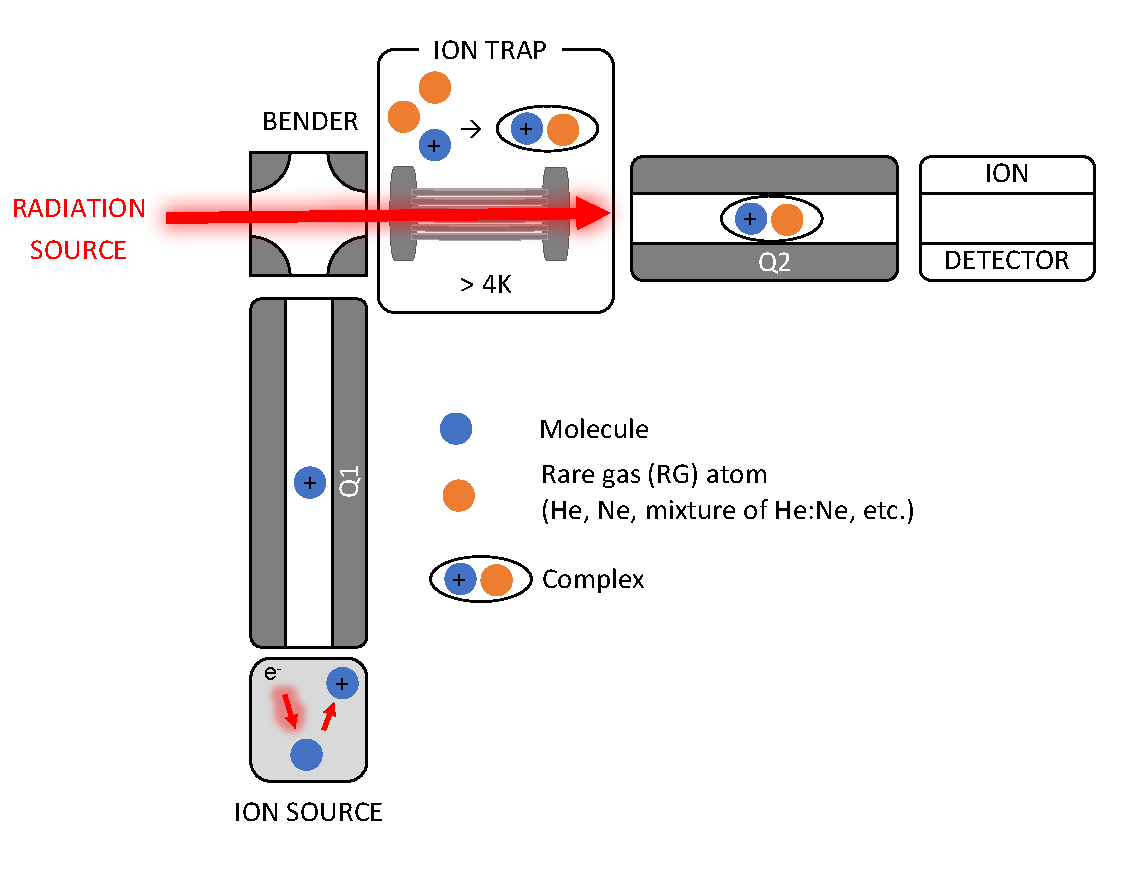
\includegraphics[width=1\textwidth]{figures/Instruments/FELion_schematics.pdf}
    
    \caption{Schematic drawing of the FELion ion trap setup. The 22-pole ion trap is coupled in-between two quadrupole mass filters (Q1 and Q2). The ions are guided into the trap from Q1 via quadruple bender (labelled BENDER). The trap contents are extracted after irradiation from the radiation source into Q2 to filter desired product molecular ions and then guided into a Daly type detector to be counted.}
    \label{fig:felion}
\end{figure}

The various spectroscopic and kinetics experimental studies reported in this thesis have been performed using the 22-pole cryogenic ion trap instrument (referred to as FELion), which has been built in the Cologne Laboratory Astrophysics group and installed permanently at the widely tunable \qt{Free Electron Lasers for Infrared eXperiments} (FELIX) \cite{oepts_free-electron-laser_1995} in Nijmegen, The Netherlands. As shown in the schematic diagram (Figure \ref{fig:felion}), the FELion instrument consists of an ion source, quadruple mass filters, an ion trap and a detector. A detailed description of the FELion instrument has been given by \citet{asvany_coltrap_2014}, \citet{kluge_state-selective_2016} and \citet{jusko_felion_2019}. This section will provide a brief discussion focusing on the FELion instrumental apparatus used in this study.

\subsection{Ion source}
\label{subsec:setup:ion-source}

One of the main challenges when studying highly reactive molecular ions is their production. The primary molecular ions are produced in the ion source using electron ionisation (EI), where an energetic electron (typical $20-70$ eV) interacts with molecules. \citet{dempster_new_1918} first demonstrated this process for the solid phase and later \citet{bleakney_new_1929} for the gas phase molecules. The ionisation process produces dissociative and non-dissociative products, i.e., ionised fragments and ionised parent molecules, respectively. A short pulse of produced ions is then extracted into the first quadrupole (Q1) by applying an adjustable pulse on the exit electrode (referred to as B0, see Figure \ref{fig:setup:ion-source}). This section will discuss the types of ion sources coupled to the FELion instrument.\\

\begin{figure}[!htb]
    \centering
    \begin{subfigure}[b]{0.49\textwidth}
        \centering
        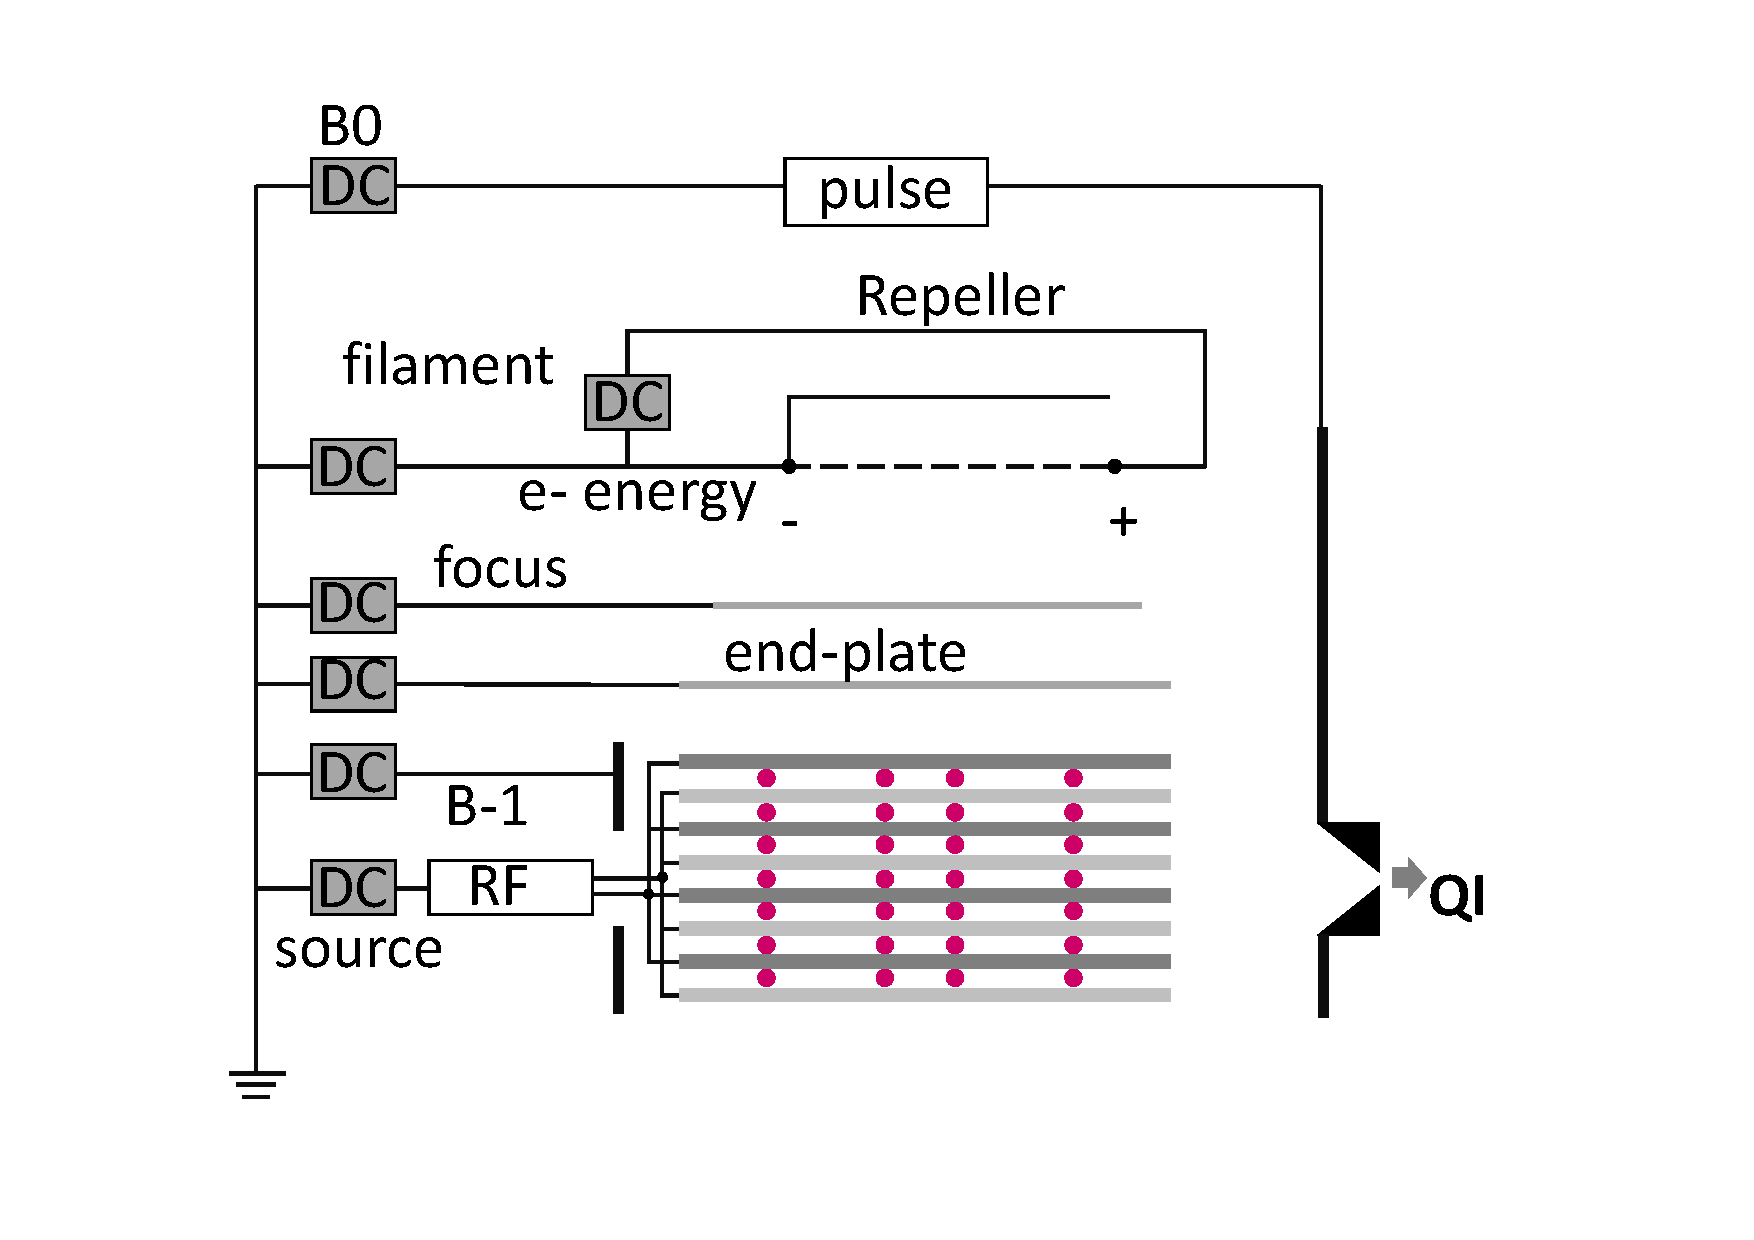
\includegraphics[width=1\textwidth]{figures/Instruments/ion-source/storage.pdf}
        \caption{}
        \label{fig:setup:storage-ion-source}
    \end{subfigure}
    \hfill
    \begin{subfigure}[b]{0.49\textwidth}
        \centering
        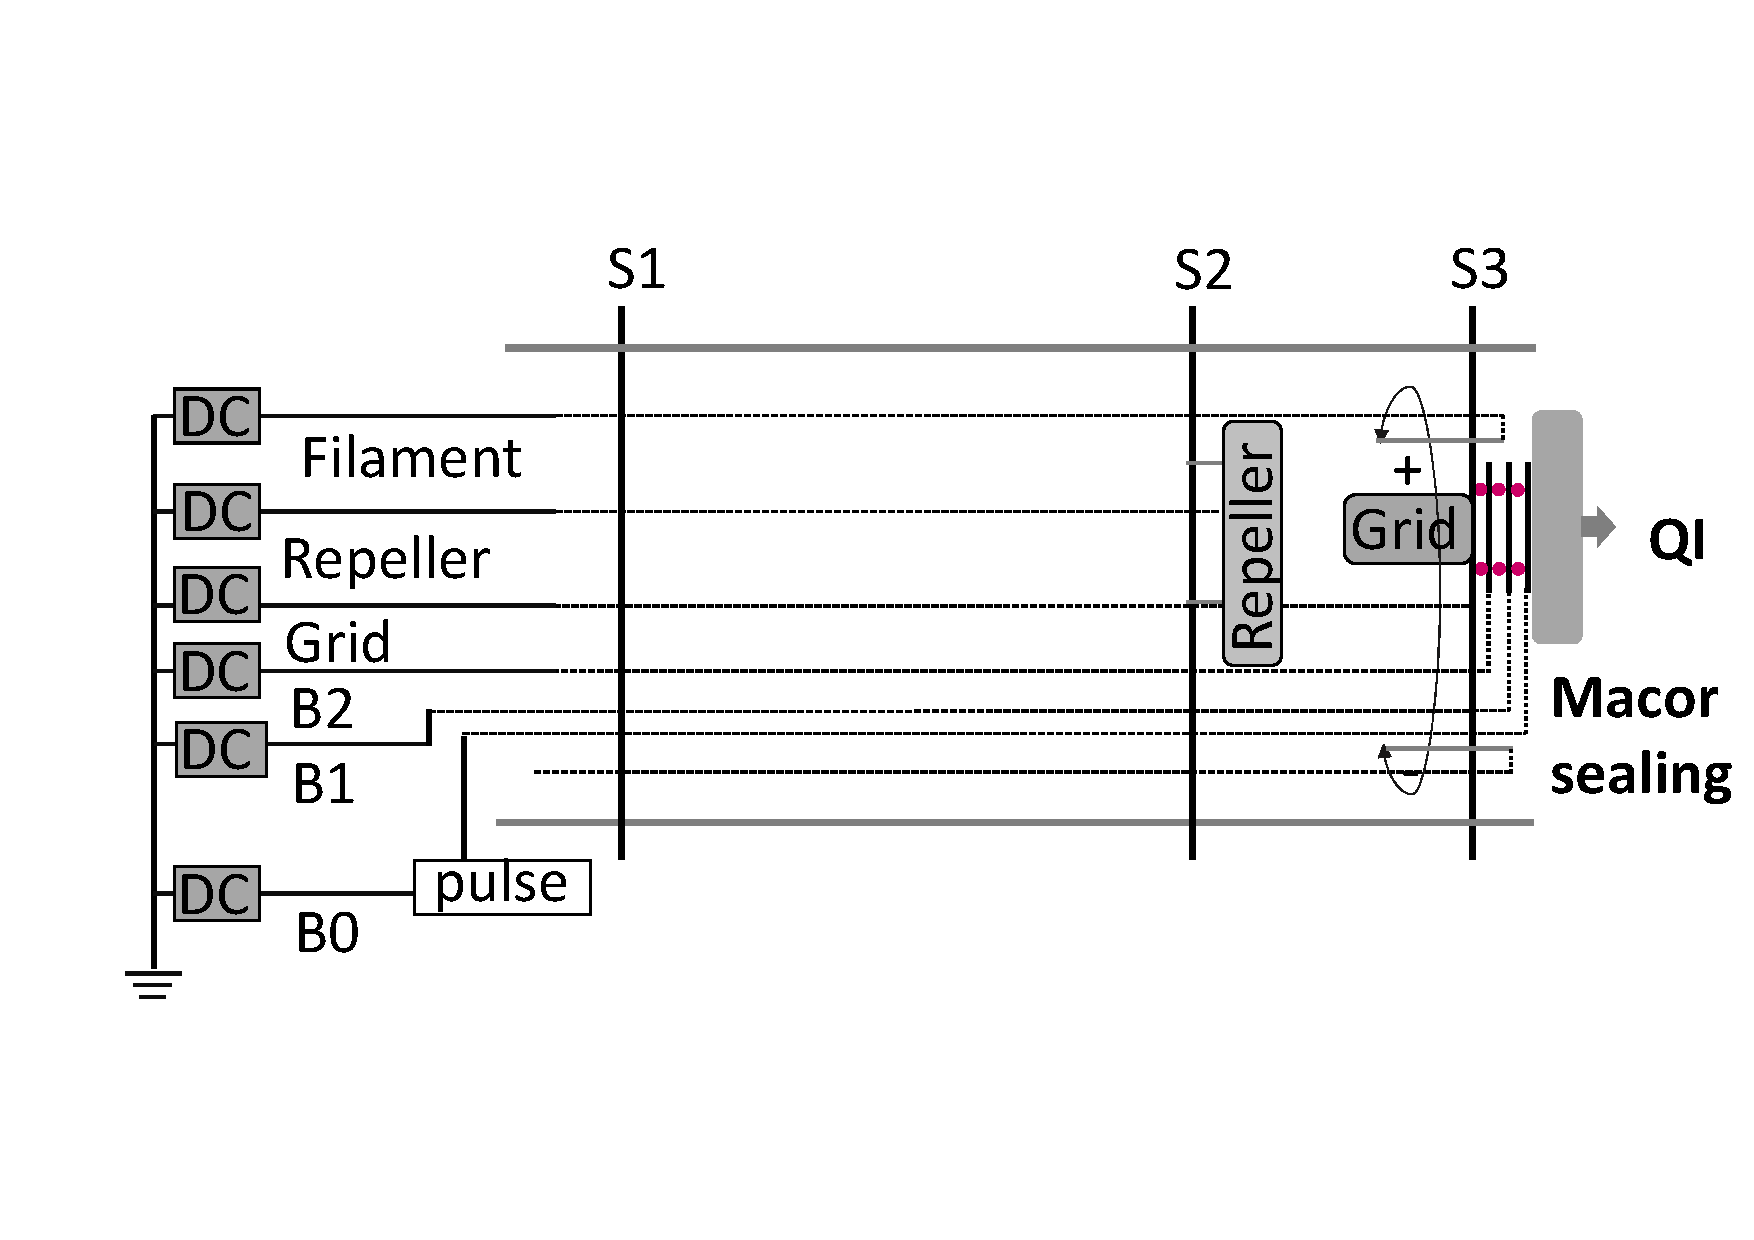
\includegraphics[width=1\textwidth]{figures/Instruments/ion-source/non-storage.pdf}
        \caption{}
        \label{fig:setup:non-storage-ion-source}
    \end{subfigure}
    \hfill
    \caption{Schematic drawing of the ion sources. The various components are labelled, and the corresponding connections are indicated by solid lines for (a) storage source and (b) non-storage (S1, S2 and S3 are grounded base plates for support). The pink circles represent ruby balls for insulation between connected electrodes. The labelled Macor sealing ring on top of the B0 electrode is placed to seal the ion source chamber and prevent any accidental contact between B0 and the Q1 rods.}
    \label{fig:setup:ion-source}
\end{figure}

\textbf{Storage source:} One type of ion source is a radiofrequency storage source, developed by \citet{gerlich_experimental_1992}. The primary ions are generated and stored ($\sim $s) in this source using an in-homogeneous RF field and DC potentials. The benefit of storing the ions in the source is that the produced molecular ions can undergo collisions with the background neutral gas or gas mixtures (typically at pressures of $10^{-6} - 10^{-5}$ mbar and a temperature of $\sim$ 400 K), leading to the production of secondary ions via chemical reactions and de-excitation and thermalization of the ions. 

As depicted in the schematic diagram (Figure \ref{fig:setup:storage-ion-source}), the storage ion source consists of a stack of eight \qt{double H-shaped} molybdenum plates (1 mm thickness), which are connected and electrically insulated by ruby balls (1 mm diameter). Four of the eight plates are connected alternately, and a typical $50-280$ V RF voltage is applied. The filament wire (rhenium $99.97 \%$, 0.2 mm diameter) is covered by the \qt{repeller} and the \qt{focus}, which are made up of 0.5 mm thick molybdenum plates. The filament typically operates around $\sim$ 5 V and 2.8 A and is held on a negative potential corresponding to the electron energy. The repeller is connected to the negative end of the corresponding filament. The DC voltages applied to the \qt{focus} and \qt{repeller} help to focus and accelerate electrons into the source. The B0 and B-1 are mounted at the front and back of the source apertures, respectively. This combination helps to confine the ions in the axial direction of the source by applying corresponding DC-potentials. The B0 can be pulsed to generate a short pulse (typically 10-100 ms) of ions for the experiments.

\textbf{Direct EI source:} The other type of ion source is called \qt{direct EI}, which produces primary ions by \qt{direct electron ionisation} but they are not stored. This source is a simple combination of repeller, grid, filament and lens, as shown in Figure \ref{fig:setup:non-storage-ion-source}. The filament wire is made up of a 0.25 mm Rhenium wire mounted in a circular arrangement around the grid covering 270 deg arc length. The filament's power supply ($\sim$ 5 V / 2.8 A) is floated to $10-70$ eV and, together with the grid voltage ($1-4$ V), acts as an electron gun which accelerates the electrons to provide the necessary energy to ionise molecules in the grid region. The repeller (typically operated around $-5 to -15$ V) is mounted on a grounded base plate with ceramic insulators and helps to focus and accelerate electrons into the grid region. The einzel lens (electrodes) set up towards the end consists of B0, B1 and B2 electrodes (insulated by ruby balls) to confine the ions in the axial direction of the source by applying corresponding DC-potentials.

Depending on the nature of the study, storage and direct EI sources can be used accordingly. The storage ion source provides the benefit of storing the formed ion for a few seconds, thereby often quenching ions to the most stable isomeric form  and the electronic ground state by undergoing (reactive) collision with the background gas. Additionally, the storage source can produce secondary ions via reactions with the background gas, e.g., protonation reactions. An efficient protonation process is, for example, discussed in more detail in chapter \ref{chapter:CH3CNH+}. On the other hand, the direct EI source allows us to produce also energetically higher-lying isomeric forms of ions and to characterize, for example, their formation routes via dissociative ionization. In Chapter \ref{chapter:C3H3+}, a detailed investigation of two different isomers (cyclic and linear form) are discussed using both direct EI and storage ion source.

Once the ions are formed in the source, a short pulse of ions is extracted into the first quadrupole mass filter (Q1). Adjusting the RF and DC potential voltages can further isolate and guide the molecular ion of interest into the trap, as will be discussed in the following section.

\subsection{Ion trap and detector}
\label{subsec:setup:ion-trap-and-detector}

The heart of the FELion instrument is a 4 K cryogenic 22-pole ion trap coupled in-between two quadrupole mass filters (Q1 and Q2). The Q1 and Q2 are perpendicularly angled. Therefore, the produced mass-filtered target ions from Q1 are guided into the trap by passing via a quadrupole bender, as shown in Figure \ref{fig:felion}. The 22-pole ions trap's design details are described by \citet{asvany_note_2010}. The trap RF is generated using amplified output (10 W amplifier) of a direct digital synthesizer (DDS) and operated at the trap resonance of around $\sim 18.3$ MHz. 

\begin{figure}[!b]
    \centering
    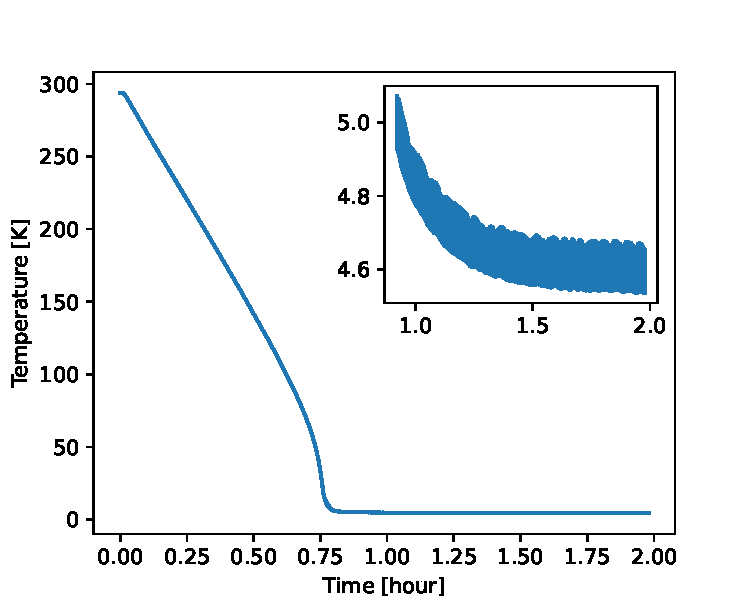
\includegraphics[width=0.9\textwidth]{figures/Instruments/cooldown-behaviour.pdf}
    \caption{Cool-down behaviour of the 22-pole cryogenic ion trap from room temperature using a He cryostat. The inset shows a detailed view of temperatures below 5 K.}
    \label{fig:cooldown_behaviour}
\end{figure}

The ion trap is mounted inside a copper housing and directly onto a cold head (Sumitomo RDK-408D2), allowing to cool it down to a minimum temperature of around 4 K using a He cryostat (see Figure \ref{fig:cooldown_behaviour}). The FELion instrument's 1 Hz machine cycle is synchronised with the cold head and FELIX laser (see Section \ref{subsec:ir:radiation-source}) for infrared experiments. The temperature can be varied between $4-40$ K using a thermo-strip (Kapton material, providing up to 40 W heating power) and monitored using an attached Si diode (Lakeshore DT-470-CU-13). The ions are kinetically and internally cooled by collisions with buffer gas atoms such as He or He:Ne mixture. However, it should be noted that the ion temperature is typically higher than the nominal trap temperature \cite{endres_incomplete_2017} (see Section \ref{subsec:collisional-ion-temperature}). The buffer gas is admitted directly into the trap region at high number densities ($10^{14}-10^{15}$\percc, see Section \ref{subsec:numer-density} for number density measurements inside trap) either continuously or via a pulsed piezo valve depending on the experimental methods. 

The ions can be stored in the trap for up to 10 s (depending on the experiment) and then extracted from the trap. Subsequently the parent or possible product ions are mass-selected with a second quadrupole mass filter (Q2) into a single-ion counting Daly type detector \cite{daly_scintillation_1960} for analysis. The pulses generated by the detector are amplified and discriminated (Phillips Scientific model 6906, 300 MHz) and counted with a gated 100 MHz counter (Ortec model 996).

In the next section, we shall discuss the spectroscopic methods employed in the 22-pole cryogenic ion trap (FELion instrument) for vibrational and rotational transition measurements of molecular ions.
